% !TeX TS-program = xelatex

\documentclass[11pt, a4paper]{report}

% Dokumentum adatok
% =================
\author{}
\title{Műszaki áramlástan feladatgyűjtemény}

% A közös fájlok beszúrása
% ========================
\newcommand*{\JakiFolder}{./JAKI}%

% A közös fájlok a JAKI tárolóban vannak, amit az MHFGY-vel 
% közös mappába kell letölteni (clone/pull).

% A "book" dokumentumosztály fölösleges oldalakat szúr be a címoldal
% és a tartalomjegyzék után.

\usepackage[utf8]{inputenc}
\usepackage[magyar]{babel}

% XeLaTeX ékezetes betűk
\usepackage{fontspec}

% A margók beállítása, később a 
%	\newgeometry{left=3cm,bottom=0.1cm}
% és a 
%	\restoregeometry
% parancsokkal egyedileg módosíthatók a margók
\usepackage[left=2cm, right=2cm, top=2cm, bottom=2cm]{geometry}

\usepackage{amsmath}
\usepackage{amssymb}

% A dupla betűk betűtípusának beállítása
\AtBeginDocument{
	\DeclareSymbolFont{AMSb}{U}{msb}{m}{n}
	\DeclareSymbolFontAlphabet{\mathbb}{AMSb}
}

% A régi német betűtípusok támogatása (fraktúra, Schwabacher, gót)
% A gót betűtípus nem működik
% Az ékezetes betűk csak a Table 18: Text-mode Accents táblázat szerint működnek
\usepackage{yfonts}

% Tabu hiba kezelés
\usepackage{booktabs}% http://ctan.org/pkg/booktabs
\newcommand\tabitem{\makebox[1em][r]{\textbullet~}}
\usepackage{tabto}
\usepackage{tabu}

% Bekeretezett részek
\usepackage[framemethod=tikz]{mdframed}
% Megjegyzés
\newcommand{\comment}[2][black!10]{%
\begin{mdframed}[hidealllines=true, backgroundcolor=#1, innerleftmargin=3pt, innerrightmargin=3pt, leftmargin=-3pt, rightmargin=-3pt]
Megjegyzés: #2
\end{mdframed}
}

%\usepackage{titlesec}

\pagestyle{plain}

\usepackage{float}
\usepackage{xifthen}

% Tizedesvessző
\usepackage{icomma}

% Függelék

\usepackage[toc,titletoc,page]{appendix}
\renewcommand{\appendixtocname}{Függelékek}
\renewcommand{\appendixpagename}{Függelékek}


%\fontspec{Times New Roman}
%\setmonofont{Consolas}
%\setmainfont{Calibri}

\usepackage{commath}
% A \Dif esetén a hatványkitevők rálógnak a D-re.
% A deriváltakban a d után sok az üres hely.

% This package will provide a complete implementation of 
% unicode maths for XELATEX and LuaLATEX.
% A Cambria Math támogatott.
% Javítja a vektor jelek elhelyezését a betűk felett.
% Az alsó és felső indexek betűtípusait módosítja, és szélesebbek a betűk.
\usepackage[math-style=TeX]{unicode-math}
%\setmathfont{XITS Math} % Túl vastagok a betűk
%\setmathfont{Cambria Math}

\usepackage{siunitx}
\sisetup{
	per-mode = fraction,
	fraction-function = \dfrac,
	detect-family = true,
	output-decimal-marker = {,},
	space-before-unit = true,
	use-xspace = true,
	exponent-product = \cdot,
	sticky-per = true
}

\usepackage[makeroom]{cancel}

% Többrészes ábrák létrehozása, subfigure környezet
\usepackage[justification=centering]{caption}
\usepackage{subcaption}

% A Hyperref csomagot lehetőleg utolsóként kell betölteni.
\usepackage[colorlinks=false]{hyperref}

% A címsorok másolása a kereszthivatkozásokba
\usepackage{nameref}

% Bekarikázott számok
\usepackage{pifont}

% Kiemelés színnel
\usepackage{xcolor}

% Az oszlopvektorok és mátrixok jelölésére
\usepackage{accents}
\newcommand{\ubar}[1]{\underaccent{\bar}{#1}}

% Színes táblázat, a tabuhoz nem szükséges
%\usepackage{colortbl}

% Fekvő oldalak
% If you are using pdfLaTeX, you should use pdflscape instead. The pdflscape package adds PDF support to the landscape environment of package lscape, by setting the PDF/Rotate page attribute. Pages with this attribute will be displayed in landscape orientation by conforming PDF viewers:
\usepackage{pdflscape}

% Kiemelés
% Több sorba osztásnál %-ezni kell a sortöréseket
%\newcommand{\highlight}[2]{\colorbox{#1}{$\displaystyle#2$}}

% Függőleges távolságok
\newcommand{\reducedstrut}{\vrule width 0pt height 1.2\ht\strutbox depth 0.95\dp\strutbox\relax}
\newcommand{\highlight}[2]{%
  \begingroup
  \setlength{\fboxsep}{1pt}% Vízszintes távolság
  \colorbox{#1}{\reducedstrut$\displaystyle#2$\/}%
  \endgroup
}

% Sortáv módosítás
\usepackage{setspace}
%\singlespacing
%\onehalfspacing
%\doublespacing

% Felsorolások
\usepackage{enumitem}

% Megjegyzés létrehozás
%\newlist{notes}{enumerate}{1}
%\setlist[notes]{label=Megjegyzés: , leftmargin=*}

% Külső fájlok írása
% Elvileg szükségtelen
%\usepackage{filecontents}

% Forráskezelés
%When using babel or polyglossia with biblatex, loading csquotes is recommended to ensure that quoted texts are typeset according to the rules of your main language.
\usepackage{csquotes}
\usepackage[ 
	backend=biber, 
	url=false, 
	citestyle=numeric,%draft,
	bibstyle=numeric,%style=numeric,%authoryear,%numeric, 
	giveninits=true, 
	clearlang=true, 
	bibencoding=auto,
	sorting=none]{biblatex}
	
\makeatletter

\newrobustcmd*{\parentexttrack}[1]{%
  \begingroup
  \blx@blxinit
  \blx@setsfcodes
  \blx@bibopenparen#1\blx@bibcloseparen
  \endgroup}

\AtEveryCite{%
  \let\parentext=\parentexttrack%
  \let\bibopenparen=\bibopenbracket%
  \let\bibcloseparen=\bibclosebracket}

\makeatother


% Az egyenletek előtti és utáni térközök beállítása
% A TikZ blokkdiagamban a 3. szinttől lefele fölösleges bal margót hoz létre (???)
%
% => NE LEGYEN ÜRES SOR AZ EGYENLETEK ELŐTT!
%
%\makeatletter
%\g@addto@macro\normalsize{%
%	\setlength\abovedisplayskip{6pt}
%	\setlength\belowdisplayskip{12pt}
%	\setlength\abovedisplayshortskip{0pt}
%	\setlength\belowdisplayshortskip{12pt}
%}
%\makeatother

% Az árva- és özvegysorok büntetése (nem biztos, hogy nem lesznek...)
\widowpenalty10000
\clubpenalty10000


% SAJÁT PARANCSOK LÉTREHOZÁSA
% ===========================

\DeclareMathOperator{\tr}{tr}

% Gradiens, forráserősség, örvényerősség
\newcommand{\Grad}[1] {\mathrm{grad\,} #1}
\newcommand{\Div}[1] {\mathrm{div\,} #1}
\newcommand{\Rot}[1] {\mathrm{rot\,} #1}
\newcommand{\Diag}[1] {\mathrm{diag\,} #1}

% Függvények
\newcommand{\Det}[1] {\mathrm{det} #1}
\DeclareMathOperator{\tg}{tg}
\DeclareMathOperator{\sgn}{sgn}
\DeclareMathOperator{\arctg}{arctg}
\DeclareMathOperator{\arctgNN}{arctg2}

% Mátrix belső közei
\makeatletter
\renewcommand*\env@matrix[1][\arraystretch]{%
	\edef\arraystretch{#1}%
	\hskip -\arraycolsep
	\let\@ifnextchar\new@ifnextchar
	\array{*\c@MaxMatrixCols c}}
\makeatother

% Oszlopvektor, sorvektor és mátrix jelölések
\newcommand{\mat}[1] {\underline{\underline{#1}}\reducedstrut}
\newcommand{\cvec}[1] {\underline{#1}\reducedstrut}
%\def\rvec#1{\underline{#1}^{T}}
%\def\mat#1{\underline{\underline{#1}}}
%\def\mat3#1{\underline{\underline{\underline{#1}}}}

\newcommand{\vektor}[2][1]{\begin{bmatrix}[#1] #2 \end{bmatrix}}
\newcommand{\tmb}[2][2]{\begin{bmatrix}[#1] #2 \end{bmatrix}}
\newcommand{\vek}[4][1]{\begin{bmatrix}[#1] #2 \\ #3 \\ #4 \end{bmatrix}}
\newcommand{\mtrx}[1]{\begin{bmatrix}#1\end{bmatrix}}



% FÜGGELÉK TARTALOMJEGYZÉK
% Appendix csomag (appendix.sty)
%\newcommand{\@redotocentry@pp}[1]{%
%  \let\oldacl@pp=\addcontentsline
%  \def\addcontentsline##1##2##3{%
%    \def\@pptempa{##1}\def\@pptempb{toc}%
%    \ifx\@pptempa\@pptempb
%      \def\@pptempa{##2}\def\@pptempb{#1}%
%      \ifx\@pptempa\@pptempb
%\oldacl@pp{##1}{##2}{##3}%A kísérleti változat: \oldacl@pp{##1}{##2}{\appendixname\space [##1][##2][##3] (\@car \splitlist{##3}\@nil) (\@cdr \splitlist{##3}\@nil)}%
%      \else
%        \oldacl@pp{##1}{##2}{##3}%
%      \fi
%    \else
%      \oldacl@pp{##1}{##2}{##3}%
%    \fi}
%}


% VÁLTOZÓK
\makeatletter
\let\JakiTitle\@title
\let\JakiAuthor\@author
\makeatother

% OLDALSZÁMOZÁS
% Oldalszámozás váltás a kezdő, a fő és a befejező szakasz határán
% A "report" osztályban nincs, a "book" osztályból másolva...
%https://tex.stackexchange.com/questions/154646/is-there-an-easy-way-to-get-the-frontmatter-mainmatter-and-backmatter-in-a-l
\makeatletter
\newcommand\frontmatterreport{%
	\cleardoublepage
	%\@mainmatterfalse
	\pagenumbering{Roman}}

\newcommand\mainmatterreport{%
	\cleardoublepage
	%\@mainmattertrue
	\pagenumbering{arabic}}

\newcommand\backmatterreport{%
	\if@openright
		\cleardoublepage
	\else
		\clearpage
	\fi
	% \@mainmatterfalse
	}
\makeatother


% HYPERREF
\hypersetup{
	pdftitle={\JakiTitle}, 
	pdfauthor={\JakiAuthor}, 
	colorlinks = true,
	citecolor = orange,
	filecolor = red,
	linkcolor = blue,
	urlcolor = red
}


% Az átmérőjel alapvonalra emelése
%\makeatletter
%\let\olddiameter\diameter
%\renewcommand{\diameter}[0]{\raisebox{\depth}{\olddiameter}}
%\makeatother

				% Formázás, csomagok

% TikZ - Ábrázolás
% ================
\usepackage{tikz} 
\usepackage{tikz-3dplot}
\usetikzlibrary{arrows.meta, automata, bending, calc, decorations.markings, fit, graphs, intersections, patterns, positioning, scopes, shapes, shapes.geometric, shapes.multipart, trees}
% bending: a nyílfejek "elnyomják" az íveket, ez a könyvtár helyre teszi...

\usepackage{pgfplots}
\pgfplotsset{compat=1.10}
\usepgfplotslibrary{fillbetween}

% Szögek méretezése
% =================

\pgfkeys{/tikz/.cd, % to set the path
	xa/.initial=0, % initial value
	xa/.get=\xa, % to get the value from a macro
	xa/.store in=\xa, % to store the value into a macro
	xb/.initial=0,
	xb/.get=\xb,
	xb/.store in=\xb,
	ya/.initial=0,
	ya/.get=\ya,
	ya/.store in=\ya,
	yb/.initial=0,
	yb/.get=\yb,
	yb/.store in=\yb,
	ra/.initial=1.25 cm,
	ra/.get=\ra,
	ra/.store in=\ra,
	rb/.initial=1.5 cm,
	rb/.get=\rb,
	rb/.store in=\rb,
	rm/.initial=0.5cm,			% \pgfangle: sugár a méretvonal töréspontjáig
	rm/.get=\rm,
	rm/.store in=\rm,
	a/.initial=0,				% \pgfangle: szög (honnan); \pgflength: nyílfej van/nincs
	a/.get=\a,
	a/.store in=\a,
	b/.initial=45,				% \pgfangle: szög (hova); \pgflength: nyílfej van/nincs
	b/.get=\b,
	b/.store in=\b,
	lv/.initial=45,
	lv/.get=\lv,
	lv/.store in=\lv,
	lm/.initial=0.5,
	lm/.get=\lm,
	lm/.store in=\lm,
	alim/.initial=0,			% \pgflength: 0/[1] bal és jobb méretsegédvonal
	alim/.get=\alim,
	alim/.store in=\alim,
	blim/.initial=0,
	blim/.get=\blim,
	blim/.store in=\blim,
	ny/.initial=1,				% \pgflength: 0/[1] a méret elforgatása (csak függőleges esetben)
	ny/.get=\ny,				% \pgfangle: nyíl/kör kiosztás
	ny/.store in=\ny,
	szín/.initial=black,
	szín/.get=\szín,
	szín/.store in=\szín,
	belül/.initial=0,		% \pgfangle: 0/1/2/3, \pgflength: 0/[1]/2 a méret helye
	belül/.get=\belül,
	belül/.store in=\belül,
	horgony/.initial=south west,		% \pgfangle, \pgfpont: a méret jelének/pont nevének horgonyzása
	horgony/.get=\horgony,
	horgony/.store in=\horgony,
	ztengely/.store in=\ztengely,
	xsh/.initial=0,
	xsh/.get=\xsh,
	xsh/.store in=\xsh,
	ysh/.initial=0,
	ysh/.get=\ysh,
	ysh/.store in=\ysh
	}

\newcommand{\pgfangle}[2][]{ %
	% Az alapértelmezett értékek visszaállítása
	\tikzset{alim=0, blim=0, szín=black, belül=0, ra=1.25, ny=1, rm=0.5, horgony=south, xsh=0, ysh=0}
	
	\tikzset{#1} % Az első argumentum a tulajdonságlista
	% (\xa, \ya) a szög csúcspontja
	% \ra az ív sugara, \rb a szög szárainak hossza
	
	% PÉLDA: \pgfangle[ra=1.25, a=\alf, b=0, blim=1]{$\alpha$};
	
	\tikzset{rb = \ra + 0.25} % a külső sugár
	\tikzset{lv = {\ra*abs(\b-\a)*3.14159/180}} % az ívhossz
	\tikzset{>={Triangle[length=4mm, width=1.25mm]}} % lokális nyílfej beállítás
	
	% A kezdőpont
	\coordinate (O) at (\xa, \ya);
	
	% A két szár és az ív végpontjai
	\coordinate (A) at ($(O) + (xyz polar cs: radius=\ra, angle=\a)$);
	\coordinate (U) at ($(O) + (xyz polar cs: radius=\rb, angle=\a)$);
	\coordinate (B) at ($(O) + (xyz polar cs: radius=\ra, angle=\b)$);
	\coordinate (V) at ($(O) + (xyz polar cs: radius=\rb, angle=\b)$);
	
	\ifnum\belül=0
		% Jobbra
		\pgfmathsetmacro{\ivalfa}{1.0/\ra*180/3.14159};
		\pgfmathsetmacro{\ivbeta}{0.5/\ra*180/3.14159};
	\else
		\ifnum\belül=2
			% Balra
			\pgfmathsetmacro{\ivalfa}{0.5/\ra*180/3.14159};
			\pgfmathsetmacro{\ivbeta}{1.0/\ra*180/3.14159};
		\else
			% A körcikken belül vagy külső vonalon
			\pgfmathsetmacro{\ivalfa}{0.5/\ra*180/3.14159};
			\pgfmathsetmacro{\ivbeta}{0.5/\ra*180/3.14159};
		\fi
	\fi
	
	\ifnum\ny=0
		% Az ív nyílfejek nélkül
		\draw[name path=iv, \szín] (A) arc [start angle=\a, end angle=\b, radius=\ra];
	\fi
	\ifnum\ny=1
		% Az ív nyílfejekkel
		\pgfmathparse{\lv > 1.0 ? int(1) : int(0)}
		\ifnum\pgfmathresult=1 
			% Belső nyílfejek
			\draw[name path=iv, \szín, <->] (A) arc [start angle=\a, end angle=\b, radius=\ra];
		\else
			% Külső nyílfejek
			\draw[name path=iv, \szín] (A) arc [start angle=\a, end angle=\b, radius=\ra];
			
			\draw[\szín, <-] (A) arc [start angle=\a, end angle={\a-\ivalfa}, radius=\ra];
			\draw[\szín, <-] (B) arc [start angle=\b, end angle={\b+\ivbeta}, radius=\ra];
		\fi
	\fi
	\ifnum\ny=2
		% Az ív nyílfejjel és kezdőkörrel jobboldalon
		\pgfmathparse{or(equal(\belül, 1), equal(\belül, 3))}
		\ifnum\pgfmathresult=1 
			% Belső felirat
			\pgfmathparse{\lv > 1.0 ? int(1) : int(0)}
			\ifnum\pgfmathresult=1 
				% Belső nyílfej
				\draw[name path=iv, \szín, ->] (A) arc [start angle=\a, end angle=\b, radius=\ra];
			\else
				% Külső nyílfej
				\draw[name path=iv, \szín] (A) arc [start angle=\a, end angle=\b, radius=\ra];
				
				\draw[\szín, -] (A) arc [start angle=\a, end angle={\a-\ivalfa}, radius=\ra];
				\draw[\szín, <-] (B) arc [start angle=\b, end angle={\b+\ivbeta}, radius=\ra];
			\fi
		\else
			% Külső felirat (belül = 0 vagy 2)
			\ifnum\belül=2
				% A nyílfej mindig kívül balra
				\draw[name path=iv, \szín] (A) arc [start angle=\a, end angle=\b, radius=\ra];
				\draw[\szín, <-] (B) arc [start angle=\b, end angle={\b+\ivbeta}, radius=\ra];
			\else
				\pgfmathparse{\lv > 1.0 ? int(1) : int(0)}
				\ifnum\pgfmathresult=1 
					% Belső nyílfej)
					\draw[name path=iv, \szín, ->] (A) arc [start angle=\a, end angle=\b, radius=\ra];
				\else
					% Külső nyílfej
					\draw[name path=iv, \szín] (A) arc [start angle=\a, end angle=\b, radius=\ra];
					
					\draw[\szín, -] (A) arc [start angle=\a, end angle={\a-\ivalfa}, radius=\ra];
					\draw[\szín, <-] (B) arc [start angle=\b, end angle={\b+\ivbeta}, radius=\ra];
				\fi
			\fi
		\fi
		
		% A kezdőkör jobboldalon
		\draw[black, fill=white] ({\ra*cos(\a)}, {\ra*sin(\a)}) circle[radius=0.5mm];
	\fi
	\ifnum\ny=3
		% Az ív nyílfejjel és kezdőkörrel baloldalon
		\pgfmathparse{or(equal(\belül, 1), equal(\belül, 3))}
		\ifnum\pgfmathresult=1 
			% Belső felirat
			\pgfmathparse{\lv > 1.0 ? int(1) : int(0)}
			\ifnum\pgfmathresult=1 
				% Belső nyílfej
				\draw[name path=iv, \szín, <-] (A) arc [start angle=\a, end angle=\b, radius=\ra];
			\else
				% Külső nyílfej
				\draw[name path=iv, \szín] (A) arc [start angle=\a, end angle=\b, radius=\ra];
				\draw[\szín, <-] (A) arc [start angle=\a, end angle={\a-\ivalfa}, radius=\ra];
			\fi
			
		\else
			% Külső felirat (belül = 0 vagy 2)
			\ifnum\belül=0
				% A nyílfej mindig kívül jobbra
				\draw[name path=iv, \szín] (A) arc [start angle=\a, end angle=\b, radius=\ra];
				\draw[\szín, <-] (A) arc [start angle=\a, end angle={\a-\ivalfa}, radius=\ra];
			\else
				\pgfmathparse{\lv > 1.0 ? int(1) : int(0)}
				\ifnum\pgfmathresult=1 
					% Belső nyílfej)
					\draw[name path=iv, \szín, <-] (A) arc [start angle=\a, end angle=\b, radius=\ra];
					\draw[\szín, -] (B) arc [start angle=\b, end angle={\b+\ivbeta}, radius=\ra];
				\else
					% Külső nyílfej
					\draw[name path=iv, \szín] (A) arc [start angle=\a, end angle=\b, radius=\ra];
					\draw[\szín, -] (B) arc [start angle=\b, end angle={\b+\ivbeta}, radius=\ra];
					\draw[\szín, <-] (A) arc [start angle=\a, end angle={\a-\ivalfa}, radius=\ra];
				\fi
			\fi
		\fi
		
		% A kezdőkör baloldalon
		\draw[black, fill=white] ({\ra*cos(\b)}, {\ra*sin(\b)}) circle[radius=0.5mm];
	\fi
	
	%\pgfmathparse{\lv}
	%\node[blue](X){\lv = \pgfmathresult};
	
	% Az ív felezőpontja (a "bending" könyvtárral nem kell a metszéspont...)
	%\coordinate (S) at ($(O) + (xyz polar cs: radius=2*\rb, angle={(\a+\b)/2})$);
	%\path[name path=O--S] (O) -- (S);
	%\path[name intersections={of=iv and O--S}];
	%\coordinate (T) at (intersection-1);
	% Másik módszer:
	%\draw[name intersections={of=V and O--S, by=W}][very thick,orange] (1,0) -- (W);
	
	% A méretezés pontjai
	\coordinate (P) at ($(O) + (xyz polar cs: radius=\ra, angle={(\a+\b)/2})$);
	\coordinate (Q) at ($(P) + (xyz polar cs: radius=\rm, angle={(\a+\b)/2})$);
	
	\pgfmathparse{abs(\a+\b)/2 < 90 ? int(1) : int(0)}
	\ifnum\pgfmathresult=1 
		\coordinate (R) at ($(Q) + (xyz polar cs: radius=\lm, angle=0)$);
		\coordinate (S) at ($(Q) + (xyz polar cs: radius=\lm/2, angle=0)$);
	\else
		\coordinate (R) at ($(Q) + (xyz polar cs: radius=-\lm, angle=0)$);
		\coordinate (S) at ($(Q) + (xyz polar cs: radius=-\lm/2, angle=0)$);
	\fi
	
	% A méretvonalak (alim és blim szerint)
	\ifnum\alim=1\draw[black] (O) -- (U);\fi
	\ifnum\blim=1\draw[black] (O) -- (V);\fi
	
	% A méret felirat
	\pgfmathsetmacro{\aha}{0.4/\ra*180/3.14}
	\ifnum\belül=0
		% A körcikken kívül jobbra
		\coordinate (W) at ($(O) + (xyz polar cs: radius={\ra+0.25}, angle={((\a-\aha)+(\a-\ivalfa))/2})$);
		\node[\szín, anchor={\horgony}, xshift={\xsh}, yshift={\ysh}] at (W) {#2};
	\fi
	\ifnum\belül=1
		% A körcikken belül
		\coordinate (W) at ($(O) + (xyz polar cs: radius={\rb-0.5}, angle={(\a+\b)/2})$);
		\node[\szín, anchor=center, xshift={\xsh}, yshift={\ysh}] at (W) {#2};
	\fi
	\ifnum\belül=2
		% A körcikken kívül balra
		\coordinate (W) at ($(O) + (xyz polar cs: radius={\ra+0.25}, angle={((\b+\aha)+(\b+\ivbeta))/2})$);
		\node[\szín, anchor=\horgony, xshift={\xsh}, yshift={\ysh}] at (W) {#2};
	\fi
	\ifnum\belül=3
		% Ponttal kapcsolódó külső megtört vonal vízszintes részén
		\draw[\szín] (P) -- (Q) -- (R);
		\node[\szín, anchor=\horgony, xshift={\xsh}, yshift={\ysh}] at (S) {#2};
		\fill[fill=\szín] (P) circle [radius=1pt];
	\fi
	}

% Hosszméret
% ==========

\newcommand{\pgflength}[2][]{ %
	% Az alapértelmezett értékek visszaállítása
	\tikzset{alim=1, blim=1, a=1, b=1, szín=black, belül=1, ra=0.65, rb=0.8, ny=1}
	
	\tikzset{#1} % Az első bemenet a tulajdonságlista
	% (\xa, \ya) és (\xb, \yb) a két végpont
	% \alim és \blim a két méretsegédvonal (van/nincs)
	% \a és \b a két méretnyíl (van/nincs) (A NYILAK HELYZETE ÖNMŰKÜDŐ)
	% \belül: a méret belül (1) vagy kívül (0: balra, 2: jobbra) van (A NYILAK ÖNMŰKÜDŐEK)
	% \ra és \rb a méretvonal távolsága és a méretsegédvonalak hossza (ELŐJELESEK)
	
	\pgfmathparse{\ra+sign(\ra)*0.15}
	\tikzset{rb=\pgfmathresult}
	%\show\pgfmathresult
	
	% A két méretezendő végpont
	\coordinate (A) at (\xa, \ya);
	\coordinate (B) at (\xb, \yb);
	
	% Zárójelezés
	\pgfmathsetmacro{\alfa}{atan2((\yb-(\ya)),(\xb-(\xa)))-90}
	
%	\pgfmathparse{{\xa, \ya, \xb, \yb}}
%	\show\pgfmathresult
%	\pgfmathparse{{\yb,-(\ya),(\yb-(\ya)),(\xb-\xa)}}
%	\show\pgfmathresult
%	\pgfmathparse{atan2((\yb-\ya),(\xb-\xa))}
%	\show\pgfmathresult
%	\show\alfa
	
	% A méretvonal és a méretsegédvonalak végpontjai
	\coordinate (C) at ($(A) + (xyz polar cs: radius=\ra, angle=\alfa)$);
	\coordinate (U) at ($(A) + (xyz polar cs: radius=\rb, angle=\alfa)$);
	\coordinate (D) at ($(B) + (xyz polar cs: radius=\ra, angle=\alfa)$);
	\coordinate (V) at ($(B) + (xyz polar cs: radius=\rb, angle=\alfa)$);
	
	% A méretsegédvonalak függetlenül a többi elemtől
	\ifnum\alim=1
		\draw (A) -- (U);
	\fi
	\ifnum\blim=1
		\draw (B) -- (V);
	\fi
	
	% A "belül" kulcs értéke legyen 1, ha nem 0 vagy 2
	\pgfmathparse{(\belül!=0) && (\belül!=2)}
	\ifnum\pgfmathresult=1\tikzset{belül = \pgfmathresult}\fi
	
	% A \D logikai értékké alakítása
	\pgfmathsetmacro{\D}{sqrt((\yb-(\ya))^2 + (\xb-(\xa))^2)<1.2}
	
	% A méret és a méretnyilak
	\ifnum\belül=1
		% A méret legyen belül
		\coordinate (M) at ($0.5*(C) + 0.5*(D) + (xyz polar cs: radius=0.15, angle={\alfa+180})$);
		
		\ifnum\ny=1
			\node[anchor=base, rotate={90+\alfa}] at (M) {#2};
		\else
			% Az elforgatás letiltása, ha alfa = +-90°
			\pgfmathtruncatemacro\intalfa\alfa
			\show\intalfa
			\ifnum\intalfa=0 
				\node[anchor=east, shift={(0.1, 0)}] at (M) {#2};
			\else
				\ifnum\intalfa=-180 
					\node[anchor=west, shift={(-0.1, 0)}] at (M) {#2};
				\else
					\node[anchor=base, rotate={90+\alfa}] at (M) {#2};
				\fi
			\fi
		\fi
		
		% A nyilak helyzete a rendelkezésre álló helytől függ
		\ifnum\D=1
			\coordinate (E) at ($(C) + (xyz polar cs: radius=0.6, angle={\alfa-90})$);
			\coordinate (F) at ($(D) + (xyz polar cs: radius=0.6, angle={\alfa+90})$);
			
			% A nyilak kívül, ha az \a és \b szerint kellenek
			\ifnum\a=1
				\draw[->] (E) -- (C);
			\fi
			
			\draw[-] (C) -- (D);
			
			\ifnum\b=1
				\draw[<-] (D) -- (F);
			\fi
		\else
			% Van 12 mm, belül lesznek a nyilak
			% A nyilak kívül, ha az \a és \b szerint kellenek
			\ifnum\a=1
				\ifnum\b=1
					\draw[<->] (C) -- (D);
				\else
					\draw[<-] (C) -- (D);
				\fi
			\else
				\ifnum\b=1
					\draw[->] (C) -- (D);
				\else
					\draw[-] (C) -- (D);
				\fi
			\fi
		\fi
	\else
		% A méret legyen kívül
		\ifnum\belül=0
			% Baloldal
			\coordinate (M) at ($(C) + (xyz polar cs: radius=0.4, angle={\alfa-90}) + (xyz polar cs: radius=0.15, angle={\alfa+180})$);
			\node[rotate={\alfa+90}, anchor=base east] (mrt) at (M) {#2};
			
			\coordinate (E) at ($(mrt.base west) + (xyz polar cs: radius=0.15, angle={\alfa})$);
			\coordinate (F) at ($(D) + (xyz polar cs: radius=0.6, angle={\alfa+90})$);
			
			\draw[->] (E) -- (C);
			\ifnum\b=1
				\draw[<-] (D) -- (F);
			\fi
		\else
			% Jobboldal
			\coordinate (M) at ($(D) + (xyz polar cs: radius=0.4, angle={\alfa+90}) + (xyz polar cs: radius=0.15, angle={\alfa+180})$);
			\node[rotate={\alfa+90}, anchor=base west] (mrt) at (M) {#2};
			
			\coordinate (E) at ($(C) + (xyz polar cs: radius=0.6, angle={\alfa-90})$);
			\coordinate (F) at ($(mrt.base east) + (xyz polar cs: radius=0.15, angle={\alfa})$);
			
			\draw[<-] (D) -- (F);
			\ifnum\a=1
				\draw[->] (E) -- (C);
			\fi
		\fi
		
		\draw[-] (C) -- (D);
		
	\fi
	}

% Derékszög jelölés
\newcommand{\pgfperpendicular}[1]{ %
	% Az alapértelmezett értékek visszaállítása
	\tikzset{a=0, b=90, szín=black, ra=0.25}
	
	\tikzset{#1} % Az első bemenet a tulajdonságlista
	% (\xa, \ya) a sarokpont
	% \a az egyik szög, \b = [90, -90]
	% \ra az ív sugara
	
	\draw[szín] ({\xa+\ra*cos(\a)}, {\ya+\ra*sin(\a)}) arc[radius={\ra}, start angle={\a}, end angle={\a + \b}];
	\fill[szín] ({\xa + 0.6*\ra*cos(\a+0.5*\b)}, {\ya + 0.6*\ra*sin(\a+0.5*\b)}) circle[radius=0.25mm];
	}

% Körvonal írásjel körül
\newcommand{\pgfcircled}[1]{ %
	\tikz[baseline=(char.base)]{\node[shape=circle, draw, inner sep=0pt] (char) {#1}} %
	}

% Pont rajzolása
\newcommand{\pgfpont}[2][]{ %
	% Az alapértelmezett értékek visszaállítása
	\tikzset{szín=black, ra=0.075, horgony=south west}
	
	\tikzset{#1} % Az első argumentum a tulajdonságlista
	% (\xa, \ya) a pont koordinátái
	% \ra a kereszt mérete
	
	\draw[szín, very thick] (\xa-\ra,\ya-\ra) -- (\xa+\ra,\ya+\ra);
	\draw[szín, very thick] (\xa+\ra,\ya-\ra) -- (\xa-\ra,\ya+\ra);
	
	\node[anchor=\horgony] at (\xa,\ya) {#2};
	}

% Koordinátarendszer 2D, 4 bemenet, az első elhagyható -> []
% \pgfcoordsys[xa={\xk}, ya={\yk}, alim={\lim}]{$x$}{$y$}{$z$};
\newcommand{\pgfcoordsys}[4][]{ %
	% A felhasznált alapértelmezett értékek visszaállítása
	\tikzset{xa=0, ya=0, alim=1, szín=black, ztengely=1}
	
	\tikzset{#1} % Az első argumentum a tulajdonságlista
	% (\xa, \ya) a koordinátarendszer középpontjának helye
	% \alim a tengelyek hossza
	
	% A középpont helye
	\coordinate (O) at (\xa, \ya, 0);
	
	\ifnum\ztengely=1
		% 3D
		\draw[->, szín] (O) -- (\xa+\alim, \ya, 0) node[anchor=north east, yshift={-0.1cm}]{#3}; % Y
		\draw[->, szín] (O) -- (\xa, \ya, 0+\alim) node[anchor=north west, yshift={0.1cm}]{#2}; % X
		\draw[->, szín] (O) -- (\xa, \ya+\alim, 0) node[anchor=north east]{#4}; % Z
	\else
		% 2D
		\draw[->, szín] (O) -- (\xa+\alim, \ya, 0) node[anchor=north east, yshift={-0.1cm}]{#2}; % Y
		\draw[->, szín] (O) -- (\xa, \ya+\alim, 0) node[anchor=north east]{#3}; % Z
	\fi
	
	%\pgfmathparse{\ra+sign(\ra)*0.15}
	%\tikzset{rb=\pgfmathresult}
	}


% STÍLUSOK

% Globális nyílfej alapértelmezés
% A Triangle és a Stealth valamiért rövidebb háromszög nyílfejet eredményez.
\tikzset{>={Kite[length=4mm, width=1.2mm, inset=0pt]}}

% Nyílfej hozzáadása egy vonal felezőpontjához
\tikzset{
	mid arrow/.style={
		postaction={
			decorate, 
			decoration={
				markings, 
				mark=% actually add a mark
				at position 0.5 with {
					\fill[#1] (3mm,0mm) -- (-3mm,1.2mm) -- (-3mm,-1.2mm) -- cycle; 
					} 
				}
			}
		}
	}

% Blokkstílus
\tikzset{
	blockmain/.style = {
		% The shape: 
		rectangle, 
		% The size: 
		minimum size=6mm, 
		inner sep=4mm, 
		% The border: 
		ultra thick, draw=blue!25!black!75, % 50% red and 50% black, 
		% and that mixed with 50% white 
		% The filling: 
		top color=white, % a shading that is white at the top... 
		bottom color=blue!50!black!20, % and something else 
		% Font 
		font=\Large\bfseries
		}
	}

\tikzset{
	block/.style = { 
		% The shape: 
		rectangle, 
		% The size: 
		minimum size=6mm, 
		% The border: 
		thick, draw=blue!50!black!75, 
		% and that mixed with 50% white 
		% The filling: 
		top color=white, % a shading that is white at the top... 
		bottom color=blue!25!black!25
		}
	}
	
% Szaggatottvonal-stílus zárt görbékhez
% https://tex.stackexchange.com/questions/214400/tikz-dashes-and-closed-curves
\tikzset{
	cycled dash pattern/.code args={on #1 off #2}{
		% Use csname so catcode of @ doesn't have do be changed.
		\csname tikz@addoption\endcsname{%
			\pgfgetpath\currentpath%
			\csname pgf@decorate@parsesoftpath\endcsname{\currentpath}{\currentpath}%
			% Length of path
			\pgfmathparse{\csname pgf@decorate@totalpathlength\endcsname}\let\lc=\pgfmathresult%
			% Length of pattern
			\pgfmathparse{#1+#2}\let\lp=\pgfmathresult%
			% Scaling factor for pattern
			\pgfmathparse{\lc/(\lp*round(\lc/\lp))}\let\f=\pgfmathresult%
			% Actually scale the pattern
			\pgfmathparse{#1*\f}\let\on=\pgfmathresult%
			\pgfmathparse{#2*\f}\let\off=\pgfmathresult%
			% Tell PGF to dash this line
			\pgfsetdash{{\on}{\off}}{0pt}}%
		}
	}

				% Rajzoló parancsok

% A dokumentum kezdete
% ====================
\begin{document}

% Címoldal
\begin{titlepage}
	\centering
	\begin{hyphenrules}{nohyphenation}
		{\scshape\LARGE Pannon Egyetem \par}
		{\scshape\LARGE Mérnöki Kar \par}
		\vspace{1cm}
		{\scshape\Large Segédlet\par}
		\vspace{1.5cm}
		\parbox{8cm}{{\centering\huge\bfseries{\JakiTitle} \par}}
		\vspace{2cm}
		{\Large\itshape\JakiAuthor\par}
		\vfill
		Műszaki áramlástan \par
		Műszaki áramlástan és hőtan I.\par
		Műszaki áramlás- és hőtan

		\vfill

		% A lap alja
		{\large \today\par}
	\end{hyphenrules}
\end{titlepage}

% Tartalomjegyzék
% A frissüléséhez általában kétszer kell lefordítani a dokumentumot
\tableofcontents


% Bevezetés
\chapter*{Alapadatok}
\addcontentsline{toc}{chapter}{Alapadatok}		% Számozatlan címsor és tartalomjegyzék-bejegyzés

\section*{A tárgy adatai}
\addcontentsline{toc}{section}{A tárgy adatai}

\begin{tabular}{ l l }
Név: & Műszaki áramlástan \\
Kód: & VEMKGEB143H \\
Kreditérték: & 3 (2 elmélet, 1 gyakorlat) \\
Követelmény típus: & vizsga \\
Szervezeti egység: & Gépészmérnöki Intézet \\
Előadás látogatása: & kötelező \\
Gyakorlat látogatása: & kötelező \\
Számonkérés: & a félév végén zárthelyi, írásbeli és szóbeli vizsga \\
\end{tabular}

\section*{A segédlet célja}
\addcontentsline{toc}{section}{A segédlet célja}

A segédlet célja.

A segédlet kidolgozása még folyamatban van.


\section*{Ajánlott szakirodalom}
\addcontentsline{toc}{section}{Ajánlott szakirodalom}

\begin{itemize}
	\item Irodalom.
\end{itemize}


% 1. fejezet
% ==========
\chapter{Hidrostatika}

% 1/1


% 1/2


% 1/3


% 1/4


% 1/5


% 1/6


% 1/7


% 1/8


% 1/9


% 1/10


% 1/11


% 1/12


% 1/13


% 1/14


% 1/15


% 1/16
\section*{1/16. feladat: Gázharang}
\addcontentsline{toc}{section}{1/16. feladat: Gázharang}
\begin{tabular}{ | p{2cm} | p{14cm} | } 
	\hline 
	Szerző & Cseresznyés Hunor, BO98IB \\
	\hline
	Szak & Biomérnök Bsc. \\
	\hline	Félév & 2019/2020 II. (tavaszi) félév  \\
	\hline
\end{tabular}
\vspace{0.5cm}

%========Feladat megfogalmazása=============

\noindent Határozza meg az ábrán látható gáztartályban uralkodó nyomást bar-ban és a gázharang súlyát,$ha$

$h = \SI{1,0}{\m}$,

$\varnothing D = \SI{3}{m}$,

$\rho_v = 10^3 kg/m^3$,

$p_0 = \SI{1}{\bar}$,

%======Ábra============
\begin{figure}[h]
\centering
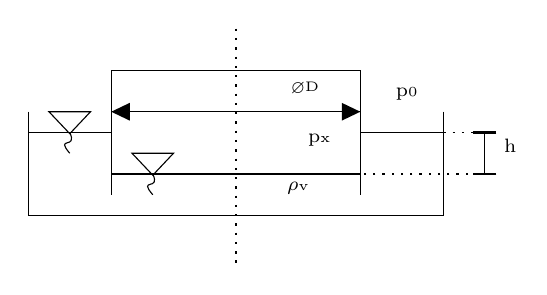
\begin{tikzpicture}[x=0.75pt,y=0.75pt,yscale=-1,xscale=1]

%========Vonal ábrázolás============== 
\draw    (260,90) -- (460,90) ;
 
\draw    (260,40) -- (260,90) ;
 
\draw    (460,40) -- (460,90) ;
 
\draw    (300,20) -- (300,80) ;

\draw    (300,20) -- (420,20) ;
 
\draw    (420,20) -- (420,80) ;
 
\draw    (300,40) -- (417,40) ;
\draw [shift={(420,40)}, rotate = 180] [fill={rgb, 255:red, 0; green, 0; blue, 0 }  ][line width=0.08]  [draw opacity=0] (8.93,-4.29) -- (0,0) -- (8.93,4.29) -- cycle    ;
 
\draw    (420,40) -- (303,40) ;
\draw [shift={(300,40)}, rotate = 360] [fill={rgb, 255:red, 0; green, 0; blue, 0 }  ][line width=0.08]  [draw opacity=0] (8.93,-4.29) -- (0,0) -- (8.93,4.29) -- cycle    ;
 
\draw [line width=0.75]  [dash pattern={on 0.84pt off 2.51pt}]  (360,0) -- (360,114) ;
 
\draw  [dash pattern={on 0.84pt off 2.51pt}]  (480.83,70) -- (420,70) ;
 
\draw  [dash pattern={on 0.84pt off 2.51pt}]  (460,50) -- (480.28,50) ;
 
\draw    (480,50) -- (480,70) ;
\draw [shift={(480,70)}, rotate = 270] [color={rgb, 255:red, 0; green, 0; blue, 0 }  ][line width=0.75]    (0,5.59) -- (0,-5.59)   ;
\draw [shift={(480,50)}, rotate = 270] [color={rgb, 255:red, 0; green, 0; blue, 0 }  ][line width=0.75]    (0,5.59) -- (0,-5.59)   ;

\draw    (260,50) -- (300,50) ;
 
\draw    (420,50) -- (460,50) ;
 
\draw    (300,70) -- (420,70) ;
 
\draw   (280.01,50.58) -- (270,40.01) -- (290,40) -- cycle ;
 
\draw    (280,50) .. controls (284,58.46) and (272.75,51.46) .. (280,60) ;
 
\draw    (320,70) .. controls (324,78.46) and (312.75,71.46) .. (320,80) ;
 
\draw   (320.01,70.57) -- (310,60) -- (330,59.99) -- cycle ;

%=========Felirat==============
\draw (385.29,24.58) node [anchor=north west][inner sep=0.75pt]  [font=\scriptsize] [align=left] {{\fontfamily{ptm}\selectfont {\tiny ⌀D}}};

\draw (435.85,26.8) node [anchor=north west][inner sep=0.75pt]  [font=\scriptsize] [align=left] {{\fontfamily{ptm}\selectfont {\scriptsize p}{\tiny 0}}};

\draw (383.46,72.4) node [anchor=north west][inner sep=0.75pt]  [font=\scriptsize] [align=left] {{\fontfamily{ptm}\selectfont {\scriptsize $\rho$}{\tiny v}}};

\draw (488,52) node [anchor=north west][inner sep=0.75pt]  [font=\scriptsize] [align=left] {{\fontfamily{ptm}\selectfont {\scriptsize h}}};

\draw (393.6,49.6) node [anchor=north west][inner sep=0.75pt]  [font=\scriptsize] [align=left] {{\fontfamily{ptm}\selectfont {\scriptsize p}{\tiny x}}};

\end{tikzpicture}
\end{figure}

%=====Feladat megoldása========
\noindent\hrulefill
\subsubsection{Feladat megoldás}
\noindent A megoldásunkhoz felhasználjuk a Pascal törvényt,amely azt mondja ki, hogy zárt térben lévő folyadékban vagy gázban a külső erő okozta nyomás minden irányban gyengítetlenül tovaterjed.

\begin{equation}
p_x = p_0+\rho_v\cdot{h}\cdot{g}
\end{equation}

\noindent Helyettesítsünk be az egyenletbe a megadott adataink alapján úgy, hogy 1 bar = 101325 Pa és a nehézségi erőt $g = 10 m/s^2$ vesszük.

\begin{equation}
p_x = 101325+\SI{e3}\cdot{1}\cdot{10} = 111325 Pa 
\end{equation}

\begin{equation}
p_x =\frac{111325}{101325}= 1,098 bar 
\end{equation}

\noindent Tehát a gáztartályban uralkodó nyomás végeredménye bar-ban: $\underline{\underline{1,098 bar}}$

\vspace{0.5cm}

\noindent Figyelnünk kell arra hogy a test(harang) vízbe merülő része egy kör alakú felület így ezzel is el kell számolnunk,tehát a gáz harang súlyát a következőképp számolhatjuk ki:

\begin{equation}
G =\frac{D^2\cdot{\pi}}{4}\cdot{h}\cdot{\rho_v}\cdot{g}
\end{equation}

\begin{equation}
G =\frac{3^2\cdot{\pi}}{4}\cdot{1}\cdot{10^3}\cdot{10} = 70685 N
\end{equation}

\noindent Tehát a gázharang súlya: 
$\underline{\underline{70685 N}}$


% 1/17


% 1/18
\section*{1/18. feladat: Hasáb alakú tartály}
\addcontentsline{toc}{section}{1/18. feladat: Hasáb alakú tartály}
\begin{tabular}{ | p{2cm} | p{14cm} | } 
	\hline 
	Szerző & Cseresznyés Hunor, BO98IB \\
	\hline
	Szak & Biomérnök Bsc. \\
	\hline	Félév & 2019/2020 II. (tavaszi) félév  \\
	\hline
\end{tabular}
\vspace{0.5cm}

%========Feladat megfogalmazása=============
\noindent Egy négyzetes hasáb alakú tartály alapéle a= 60 cm, oldaléle l=2 m , ha $\rho= 1250  kg/m^3$ sűrűségű folyadékkal teletöltjük, mekkora az alaplapjára és az oldalfalára ható erő? $(g=9,81 m/s^2)$

%======Ábra============
\begin{figure}[h]
\centering
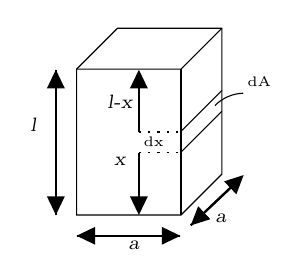
\begin{tikzpicture}[x=0.75pt,y=0.75pt,yscale=-1,xscale=1]


%=====Vonal ábrázolás=======
\draw   (310,39.72) -- (329.72,20) -- (380,20) -- (380,90.28) -- (360.28,110) -- (310,110) -- cycle ; \draw   (380,20) -- (360.28,39.72) -- (310,39.72) ; \draw   (360.28,39.72) -- (360.28,110) ;

\draw [line width=0.75]    (310,120) -- (357,120) ;
\draw [shift={(360,120)}, rotate = 180] [fill={rgb, 255:red, 0; green, 0; blue, 0 }  ][line width=0.08]  [draw opacity=0] (8.93,-4.29) -- (0,0) -- (8.93,4.29) -- cycle    ;
 
\draw [line width=0.75]    (300,110) -- (300,43) ;
\draw [shift={(300,40)}, rotate = 450] [fill={rgb, 255:red, 0; green, 0; blue, 0 }  ][line width=0.08]  [draw opacity=0] (8.93,-4.29) -- (0,0) -- (8.93,4.29) -- cycle    ;
 
\draw [line width=0.75]    (365,115) -- (388.3,92.8) ;
\draw [shift={(390.48,90.74)}, rotate = 496.4] [fill={rgb, 255:red, 0; green, 0; blue, 0 }  ][line width=0.08]  [draw opacity=0] (8.93,-4.29) -- (0,0) -- (8.93,4.29) -- cycle    ;
 
\draw [line width=0.75]    (385.48,95.74) -- (367.19,112.94) ;
\draw [shift={(365,115)}, rotate = 316.75] [fill={rgb, 255:red, 0; green, 0; blue, 0 }  ][line width=0.08]  [draw opacity=0] (8.93,-4.29) -- (0,0) -- (8.93,4.29) -- cycle    ;
 
\draw [line width=0.75]    (360,120) -- (313,120) ;
\draw [shift={(310,120)}, rotate = 360] [fill={rgb, 255:red, 0; green, 0; blue, 0 }  ][line width=0.08]  [draw opacity=0] (8.93,-4.29) -- (0,0) -- (8.93,4.29) -- cycle    ;
 
\draw [line width=0.75]    (300,40) -- (300,107) ;
\draw [shift={(300,110)}, rotate = 270] [fill={rgb, 255:red, 0; green, 0; blue, 0 }  ][line width=0.08]  [draw opacity=0] (8.93,-4.29) -- (0,0) -- (8.93,4.29) -- cycle    ;
 
\draw    (360,70) -- (380,50) ;
 
\draw    (360,80) -- (380,60) ;
 
\draw  [dash pattern={on 0.84pt off 2.51pt}]  (340,70) -- (360,70) ;

\draw  [dash pattern={on 0.84pt off 2.51pt}]  (340,80) -- (360,80) ;
 
\draw [line width=0.75]    (340,80) -- (340,107) ;
\draw [shift={(340,110)}, rotate = 270] [fill={rgb, 255:red, 0; green, 0; blue, 0 }  ][line width=0.08]  [draw opacity=0] (8.93,-4.29) -- (0,0) -- (8.93,4.29) -- cycle    ;

\draw [line width=0.75]    (340,70) -- (340,43) ;
\draw [shift={(340,40)}, rotate = 450] [fill={rgb, 255:red, 0; green, 0; blue, 0 }  ][line width=0.08]  [draw opacity=0] (8.93,-4.29) -- (0,0) -- (8.93,4.29) -- cycle    ;
 
\draw  [draw opacity=0] (376.63,57.28) .. controls (378.26,55.56) and (380.39,54.06) .. (382.9,52.97) .. controls (385.38,51.89) and (387.92,51.35) .. (390.28,51.32) -- (387.07,62.56) -- cycle ; \draw   (376.63,57.28) .. controls (378.26,55.56) and (380.39,54.06) .. (382.9,52.97) .. controls (385.38,51.89) and (387.92,51.35) .. (390.28,51.32) ;

%======Felirat=========
\draw (287.65,62) node [anchor=north west][inner sep=0.75pt]  [xslant=0.17] [align=left] {{\fontfamily{ptm}\selectfont {\scriptsize l}}};

\draw (334.72,121) node [anchor=north west][inner sep=0.75pt]  [xslant=0.2] [align=left] {{\fontfamily{ptm}\selectfont {\scriptsize a}}};

\draw (376.65,108.37) node [anchor=north west][inner sep=0.75pt]  [xslant=0.2] [align=left] {{\fontfamily{ptm}\selectfont {\scriptsize a}}};

\draw (324.69,51) node [anchor=north west][inner sep=0.75pt]  [xslant=0.16] [align=left] {{\fontfamily{ptm}\selectfont {\scriptsize l-x}}};

\draw (327.69,81) node [anchor=north west][inner sep=0.75pt]  [xslant=0.16] [align=left] {{\fontfamily{ptm}\selectfont {\scriptsize x}}};

\draw (341,71) node [anchor=north west][inner sep=0.75pt]   [align=left] {{\fontfamily{ptm}\selectfont {\tiny dx}}};

\draw (391,42) node [anchor=north west][inner sep=0.75pt]   [align=left] {{\tiny {\fontfamily{ptm}\selectfont dA}}};

\end{tikzpicture}
\end{figure}
%=====Feladat megoldása========

\noindent\hrulefill
\subsubsection{Feladat megoldás}
\noindent A nyomóerő merőlegesen hat a négyzet alakú hasáb alapjára. Ennek nagysága a nyomás és a felület nagyságának szorzatától függ. Az alapra irányuló nyomást meghatározhatjuk a folyadék sűrűségéből, a ránehezedő folyadékmagasság illetve a nehézségi erő szorzatából. Emellett definiálunk egy "A" felületelemet, aminek területe $a\cdot{a}$ lesz. Mértékegységekre figyeljünk!
\begin{equation}
F_a = p\cdot{A}=\rho\cdot{g}\cdot{l}\cdot{A}=8829 N
\end{equation}
\noindent{Tehát az alaplapjára ható erő: $\underline{\underline{8829 N}}$}

\vspace{0.5cm}

\noindent Az oldalfalára ható erő megállapításkor először válasszunk ki egy felületelemet (dA)-t és menjünk le differenciális szintre, erre a felületelemre vizsgáljuk meg a erőviszonyokat.Ha differenciális szinten eredményre jutunk, akkor terjesszük ki az egész felületelemre. Nézzük az egyenletek szempontjából:

\begin{equation}
dA= a\cdot{dx} 
\end{equation}

\begin{equation}
dF= p(x)\cdot{dA}
\end{equation}

\begin{equation}
p(x)= \rho\cdot{g}\cdot{(l-x)}
\end{equation}

\begin{equation}
\int dF =\int\rho\cdot{g}\cdot{(l-x)}\cdot{a}\cdot{dx}
\end{equation}

\begin{equation}
F =\rho\cdot{g}\cdot{a}\int_{0}^l(l-x)\cdot{dx}
\end{equation}

\begin{equation}
F =\rho\cdot{g}\cdot{a}\cdot[-\cdot(\frac{l-x}{2})^2]_{0}^l =\rho\cdot{g}\cdot{a}\cdot\frac{l^2}{2}=14715N
\end{equation}

\noindent {Tehát az oldalfalára ható erő: $\underline{\underline{14715 N}}$}

\vspace{0.5cm}


% 1/19


% 1/20


% 1/21



\chapter{Veszteségmentes csőáramlások}

% 2/1 Szódásszifon


% 2/2 Függőleges Venturi-mérő


% 2/3 Vízszintes Venturi-mérő


% 2/4 Túlnyomásos tartályrendszer


% 2/5 Vízrakéta


% 2/6 Szivornya


% 2/7 Tartály oldalán kiömlő vízsugár


% 2/8 Pipacső vízszállítása


% 2/9 Vízszintemelkedés pipacsőben


% 2/10 Csővezetékben áramló levegő


% 2/11 Áramló folyadék tömegfajlagos energiája


% 2/12 Dugattyú megengedhető legnagyobb gyorsulása


% 2/13 Forgó könyökcső vízszállítása



\chapter{Folyadékáramlás erőhatásai, kifolyás tartályból}

% 3/1 Vízsugár erőhatása


% 3/2 Ívelt lapátra érkező vízsugár


% 3/3 Éket emelő vízsugár


% 3/4 Rugót tehermentesítő vízsugár


% 3/5 Átáramlott ívcsőre ható erő


% 3/6 Bővülő ívcsőre ható erő


% 3/7 Átáramlott szűkítőre ható erő


% 3/8 Coandă-hatás


% 3/9 Megtört lapra ható erő


% 3/10 Borda-féle kifolyónyílással ellátott tartály


% 3/11 Hengeres tartály kiürülési ideje


% 3/12 Kifolyás kúpos tartályból


% 3/13 Kifolyó olaj nyúlóssága


% 3/14 Tartályok közötti vízszint-kiegyenlítődés


\chapter{Valós folyadék áramlása csővezetékben}

% 4/1 Síklap vontatás folyadékrétegen


% 4/2 Nyomásesés vizet szállító csővezetéken


% 4/3 Veszteséges áramlás részben kitöltött csatornában


% 4/4 Veszteséges áramlás gyűrű keresztmetszetű csatornában


% 4/5 Csővezetékrendszer


% 4/6 Keveredő áramlás számítása


% 4/7 Csővezetékrendszer szivattyúval


% 4/8 Pelton-turbina nyomócsövének vesztesége


% 4/9 Nyomás meghatározás csővezetékrendszerben


% 4/10 Szívócső számítása


% 4/11 Csővezeték méretezése


\chapter{Összenyomhatatlan folyadék egyméretű áramlása}

% 5/1 Pitot--Prandtl-cső


% 5/2 Billenőgyűrűs manométer


% 5/3 Venturi-mérő veszteséges számítása


% 5/4


% 5/5


% 5/6


% 5/7



\end{document}